%ifdef TWOSIDE
	%\documentclass[a4paper,12pt,final,twoside,openright]{book}
%elif ONESIDE
	\documentclass[a4paper,12pt,final,oneside]{book}
%endif

\usepackage{rapport}

\newcommand{\reporttitle}{Prolog}
\newcommand{\enseignants}{Jean~François~\textsc{Boulicaut}\\ Mehdi~\textsc{Kaytoue}}
\newcommand{\reportauthor}{Guillaume~\textsc{Abadie}\\ Nicolas~\textsc{Buisson}\\ Louise~\textsc{Crépet}\\ Rémi~\textsc{Domingues}\\ Aline~\textsc{Martin}\\ Martin~\textsc{Wetterwald}}
\newcommand{\hexanome}{H4404}
\newcommand{\reportsubject}{Livrable de projet}
\newcommand{\stagetopic}{Puissance 4}
\newcommand{\dateperiod}{du 1\up{er} au 15 octobre 2013}
\newcommand{\HRule}{\rule{\linewidth}{0.5mm}}
\setlength{\parskip}{1ex} % Espace entre les paragraphes

\hypersetup{
	pdftitle={\reporttitle},%
		pdfauthor={\reportauthor},%
		pdfsubject={\reportsubject},%
		pdfkeywords={INSA Lyon} {Prolog} {Puissance 4}
}

\title{\reporttitle}
\author{\reportauthor}
%\setcounter{tocdepth}{4}
\begin{document}
	\renewcommand{\chaptername}{} %\renewcommand{\thechapter}{}

	\pagestyle{empty}
	\pagenumbering{Roman}
	% Inspiré de http://en.wikibooks.org/wiki/LaTeX/Title_Creation
\begin{center}
	\begin{minipage}[t]{0.48\textwidth}
	  \begin{flushleft}
	    
\includegraphics [width=40mm]{images/logo_INSA.png} \\[0.5cm]
			INSA Lyon\\
			20, avenue Albert Einstein\\
			69621 Villeurbanne Cedex
	  \end{flushleft}
	\end{minipage}
	\begin{minipage}[t]{0.48\textwidth}
	  \begin{flushright}
	    %\includegraphics [width=60mm]{images/logo_Passau.jpg} \\[0.5cm]
	    %Universität Passau\\
		%Innstraße, 3\\
		%	D-94032 Passau
	  \end{flushright}
	\end{minipage} \\[2cm]

	\textsc{\Large \reportsubject}\\[0.3cm]
	\HRule \\[0.4cm]
	{\Huge \bfseries \reporttitle}\\[0.3cm]
	{\LARGE \bfseries «~\stagetopic~»}\\[0.3cm]
	{\Large \dateperiod}\\[0.4cm]
	\HRule \\[1cm]

	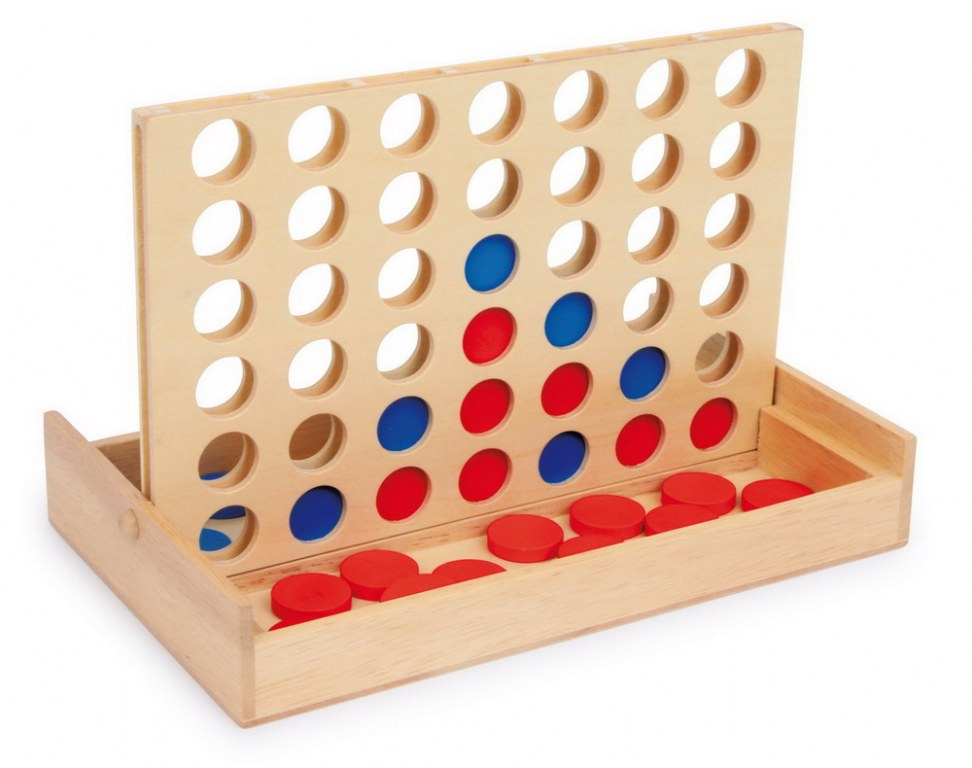
\includegraphics [scale=0.25]{images/puissance4.jpg} \\[0.7cm]
	\begin{minipage}[t]{0.4\textwidth}
	  \begin{flushleft} \large
	    \emph{Hexanôme \textbf{\hexanome}~:}\\
	    \small \reportauthor
	  \end{flushleft}
	\end{minipage}
	\begin{minipage}[t]{0.5\textwidth}
	  \begin{flushright} \large
	    \emph{Enseignants~:} \\
	    \enseignants
	  \end{flushright}
	\end{minipage}

	\vfill
	\footnotesize{Année scolaire 2013-2014}
\end{center}

	%ifdef TWOSIDE
		%\cleardoublepage
	%endif

	%% Inspiré de http://en.wikibooks.org/wiki/LaTeX/Title_Creation
\begin{center}
	\vspace*{8cm}
	\textsc{\Large \reportsubject}\\[0.3cm]
	\HRule \\[0.4cm]
	{\Huge \bfseries \reporttitle}\\[0.3cm]
	{\LARGE \bfseries «~\stagetopic~»}\\[0.3cm]
	{\Large \dateperiod}\\[0.4cm]
	\HRule \\[1cm]

	\begin{minipage}[t]{0.4\textwidth}
	  \begin{flushleft} \large
	    \emph{Hexanôme \textbf{\hexanome}~:}\\
	    \small \reportauthor
	  \end{flushleft}
	\end{minipage}
	\begin{minipage}[t]{0.5\textwidth}
	  \begin{flushright} \large
	    \emph{Enseignants~:} \\
		\enseignants
	  \end{flushright}
	\end{minipage}
\end{center}


	%ifdef 
		%  \newpage
		%	\null
		%	\vfill
	%endif

	\sloppy          % Justification moins stricte : des mots ne dépasseront pas des paragraphes



	\mainmatter
	\pagestyle{headings}

	\renewcommand{\chaptermark}[1]{\markboth{\MakeUppercase{\chaptername\ \thechapter.\ #1}}{}}
	\renewcommand{\sectionmark}[1]{\markright{\thesection{} #1}}

	\chapter{Bilan des exercices}
\section{Exercice~1}


	\chapter{Projet~: Puissance~4}

\section{Règles du jeu}
Le \texttt{Puissance~4} est un jeu de société à deux joueurs. Chaque joueur doit,
chacun son tour, insérer un jeton de sa couleur dans une des sept colonnes
du plateau de jeu, chacune ayant une capacité maximale de six jetons. On peut voir chaque colonne comme
une pile de jetons, puisqu'on ne peut qu'empiler des jetons les uns sur les autres.
Le but du jeu est d'\textbf{aligner} verticalement, horizontalement ou en diagonale \textbf{4~jetons} de sa couleur avant l'adversaire.


\section{But du joueur idéal}

Dans le cas d'un joueur idéal, le but est simplement, après avoir aligné 3~jetons,
de prévoir de jouer le 4\up{ème} au tour suivant. Mais, comme l'adversaire pourrait casser la ligne en jouant à cet endroit
lors de son tour, l'objectif du joueur idéal est donc de réaliser au moins deux alignements de 3 jetons,
laissant ainsi le joueur adverse contre l'inévitable~: il ne pourra plus contrer ces alignements en un seul jeton.


\section{Travail réalisé}

En plus de l'implémentation du module du mécanisme de jeu et de la réalisation des
tests unitaires, nous avons implémenté 4 joueurs autonomes, dont une intelligence artificielle~:
\begin{itemize}

    \item joueur aléatoire~;
    \item joueur aléatoire muni d'heuristiques~;
    \item joueur parcourant l'arbre des possibilités~;
    \item intelligence artificielle apprenant par \textbf{moteur d'inférence} de ses
    échecs précédents.\\
\end{itemize}

Mais également~:
\begin{itemize}
    \item interface utilisateur en ligne de commande pour jouer une partie~;
    \item module de tournois générant des statistiques~;
    \item module d'entrainement du moteur d'inférence~;
    \item module d'étude de l'apprentissage du moteur d'inférence~;
    \item sauvegarde et chargement de la base de connaissances du moteur d'inférence.
\end{itemize}

\end{document}
